\documentclass{beamer}

\usepackage{txfonts}
\usepackage{hyperref}
\usepackage{fancybox}
\usepackage{xfrac}
\usepackage{cancel}

\newcommand{\heart}{\ensuremath\heartsuit}

\usepackage{mathtools,amssymb}
\newcommand{\myarrow}{\scalebox{2}[2]{$\mathclap{\curvearrowleft}\mkern2.2mu
                                                 \mathclap{\curvearrowright}$}}

\DeclareMathOperator{\Bin}{\mathrm{Bin}}

\hypersetup{colorlinks=false,linkbordercolor=red,linkcolor=green,pdfborderstyle={/S/U/W 1}}

\addtobeamertemplate{navigation symbols}{}{ \hspace{1em}    \usebeamerfont{footline}%
    \insertframenumber / \inserttotalframenumber}

\geometry{papersize={15cm,12cm}}
\usepackage{lipsum}

\makeatletter
\newenvironment<>{contdproof}[1][\proofname]{%
    \par
    \def\insertproofname{#1\@addpunct{.}}%
    \usebeamertemplate{proof begin}#2}
  {\usebeamertemplate{proof end}}
\makeatother


\setbeamertemplate{theorems}[numbered]

\newtheorem*{nonumdefinition}{Definition}
\newtheorem*{nonumproblem}{Problem}
\newtheorem*{nonumtheorem}{Theorem}
\newtheorem*{nonumremark}{Remark}
\newtheorem*{answer}{Answer}
\newtheorem*{nonumremarks}{Remarks}
\newtheorem*{nonumexamples}{Examples}
\newtheorem*{nonumsolution}{Solution}
\newtheorem*{nonumexample}{Example}
\newtheorem*{nonumproposition}{Proposition}
\newtheorem{proposition}[theorem]{Proposition}


\usepackage{tikz}
\newcommand*\mycirc[1]{%
  \tikz[baseline=(C.base)]\node[draw,circle,inner sep=.7pt](C) {#1};\:
}

\newcommand\myheading[1]{%
  \par\bigskip
  {\color{blue}{\large #1}}\par\smallskip}

%\usetheme{Warsaw}
%\usetheme{Berkeley} %sample 1

\usetheme{Berlin} % sample 2
%\usetheme{AnnArbor} % sample 3

\let\otp\titlepage
\renewcommand{\titlepage}{\otp\addtocounter{framenumber}{-1}}

\title{Lecture 7}
\author{}
\date{}

\begin{document}
\begin{frame}[plain]
\titlepage
\end{frame}

\begin{frame}
\myheading{The Five Basic Discrete Random Variables}
\begin{enumerate}
\item Binomial

\item Hypergeometric

\item Geometric

\item Negative Binomial

\item Poisson
\end{enumerate}

\begin{nonumremark}
On the handout ``The basic probability distributions'' there are six distributions. I did not list the Bernoulli distribution above because it is too simple.
\end{nonumremark}

In this lecture we will do 1. and 2. above.
\end{frame}

\begin{frame}
\myheading{The Binomial Distribution}

Suppose we have a Bernoulli experiment with $P(S)=P$, for example, a weighted coin with $P(H)=P$. As usual we put $q=1-p$.

Repeat the experiment (flip the coin). Let $X=\sharp$ of successes ($\sharp$ of heads).

We want to compute the probability distribution of $X$. Note, we did the special case $n=3$ in Lecture 6, pages 4 and 5.
\end{frame}

\begin{frame}
Clearly the set of possible values for $X$ is $0,1,2,3,\ldots,n$.

Also
$$
P(X=0)=P(TT \ \ T)=qq\ldots q=q
$$

\myheading{Explanation}

Here we assume the outcomes of each of the repeated experiments are {\it independent} so
\begin{align*}
&P((T\text{~ on~ } 1^{\text{st}})\cap (T\text{~ on~ }2^{\text{nd}})\cap\cdots\cap (T\text{~ on} n\text{-th})\\[3pt]
&\quad P(T\text{~ on~ } 1^{\text{st}})P(T\text{~ on~ } 2^{\text{rd}})\ldots P(T\text{~ on~ } n\text{-th})\\[3pt]
&\quad q \ q \ldots q = q^{n}
\end{align*}
Note $T$ on $2^{\text{nd}}$ mean) $T$ on $2^{\text{nd}}$ {\it with no other information} so
$$
P(T\text{~ on~ } 2^{\text{nd}})=q.
$$
\end{frame}

\begin{frame}
Also
$$
P(X=n)=P(HH\ldots H)=P^{n}
$$
Now we have to work

What is $P(X=1)?$

\myheading{Another standard mistake}

The events $(X=1)$ and $\underbrace{HTT\ldots T}_{n-1}$ are NOT equal.

\myheading{Why - the head doesn't have to come on the first toss}

So in fact
$$
(X=1)=HTT\ldots T\cup THT\ldots T\cup\cdots\cup TTT\ldots TH
$$
\end{frame}

\begin{frame}
All of the $n$ events on the right have the same probability namely $pq^{n-1}$ and they are mutually exclusive. There are $n$ of them so
$$
P(X=1)=npq^{n-1}
$$
Similarly
$$
P(X=n-1)=npq^{n-1}
$$
(exchange $H$ and $T$ above)
\end{frame}

\begin{frame}
\myheading{The general formula}

Now we want $P(X=k)$

First we note
$$
P(\underbrace{H\ldots H}_{k} \ \underbrace{TT\ldots T}_{n-k})=p^{k}q^{n-k}
$$
But again the heads don't have to come first. So we need to
\begin{itemize}
\item[(1)] Count all the words of length $n$ in $H$ and $T$ that involve $k$. It's and $n-k$ $T$'s.

\item[(2)] Multiply the number in (1) by $p^{k}q^{n-k}$.
\end{itemize}
\end{frame}

\begin{frame}
So how do we solve 1. Think of filling $n$ slot's with the $H$'s and $n-k$ $T$'s
$$
\underbrace{\underline{~~~} \ \ \underline{~~~} \ \ \underline{~~~} \ \ \underline{~~~} \ \ \underline{~~~} \ \ \underline{~~~} \ \ \underline{~~~}}
$$

\myheading{Main Point} 

Once you decide where the $kH$'s go you have no choice with the $T$'s. They have to go in the remaining $n-k$ slots.

So choose the $k$-slots when the heads go. So we here to make a choose of $k$ things from $n$ things so $\binom{n}{k}$.
\end{frame}

\begin{frame}
So,
$$
P(X=k)=\binom{n}{k}P^{k}q^{n-k}
$$
So we have motivated the following definition.

\begin{nonumdefinition}
A discrete random variable $X$ is said to have binomial distribution with parameters $n$ and $p$ (abbreviated $X \sim \Bin(n,p)$)

If $X$ takes values $0,1,2,\ldots,n$ and
\begin{equation*}
P(X=k)=\binom{n}{k}p^{k}q^{n-k},0\leq k\leq n.\tag{*}
\end{equation*}
\end{nonumdefinition}
\end{frame}

\begin{frame}
\begin{nonumremark}
The text uses $x$ instead of $k$ for the independent (i.e., input) variable. So this would be written
$$
P(X=x)=\binom{n}{x}p^{x}q^{n-x}
$$
I like to save $x$ for the case of continuous random variables.
\end{nonumremark}

Finally we may write
\begin{equation*}
P(k)=\binom{n}{k}p^{k}q^{n-k}, \ \ 0\leq k\leq n\tag{**}
\end{equation*}
The text uses $b(\cdot,n,p)$ for $p(\cdot)$ so would write for (**)
$$
b(k,n,p)=\binom{n}{k}p^{k}q^{n-k}
$$
\end{frame}

\begin{frame}
\myheading{The Expected Value and Variance of a Binomial Random Variable}

\begin{nonumproposition}
Suppose $X \sim \Bin (n,p)$. Then $E(X)=np$ and $V(X)=npq$ so $\sigma$ = standard deviation $=\sqrt{npq}$.
\end{nonumproposition}

\begin{nonumremark}
The formula for $E(X)$ is what you might expect. If you toss a fair coin 100 times the $E(X)=$ expected number of heads $np=(100)\left(\dfrac{1}{2}\right)=50$.

However if you toss it 51 times then $E(X)=\dfrac{51}{2}$ - not what you ``expect''.
\end{nonumremark}
\end{frame}

\begin{frame}
\myheading{Using the binomial tables}

Table A1 in the text

pg. 664-666 tabulates the cdf $B(x,n,p)$ for $n=5,10,15,20,25$ and selected values of $p$.

\begin{nonumexample}[3.32]
Suppose that 20\% of all copies of a particular text book fail a certain binding strength text. Let $X$ denote the number among 15 randomly selected copies that fail the test. Find
$$
P(4\leq X\leq 7).
$$
\end{nonumexample}
\end{frame}

\begin{frame}
\begin{nonumsolution}
$X\sim \Bin (15,.2)$. We wont to compute $P(4\leq X\leq 7)$ using the table on page 664. So how to we write $P(4=leq X\leq 7)$ in terms of terms of the form $P(X\leq a)$ 

\medskip
\centerline{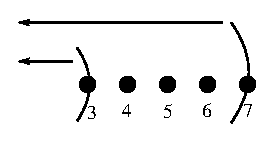
\includegraphics{figure/fig1.eps}}
\smallskip
\end{nonumsolution}

\begin{answer}
$$
(\sharp) P(4\leq X\leq 7)=P(X\leq 7)-P(X\leq 3)
$$
So
$$
P(4\leq X\leq 7)=B(7,.15,.2)-B(3,.15,.2)
$$
from table
$$
=.996-.648
$$
{\bf N.B.} {\it Understand $(\sharp)$.} This the key using computers and statistical calculators to compute.
\end{answer}
\end{frame}

\begin{frame}
\myheading{The hypergeometric distribution}

\begin{nonumexample}

\centerline{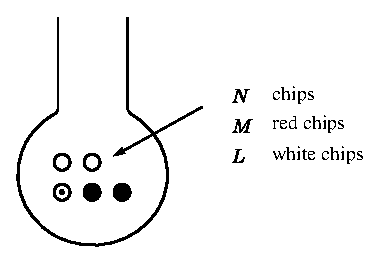
\includegraphics{figure/fig2.eps}}

Consider an urn containing $N$

Chips of which $M$ are red and $L=N-M$ are white. Suppose we remove $n$ chips {\it without replacement} so $n\leq N$. 

Define a random variable $X$ by $X=\sharp$ of red chips we get.
\end{nonumexample}
\end{frame}

\begin{frame}
Find the probability distribution of $X$.

\begin{nonumproposition}
\begin{equation*}
P(X=k)=\dfrac{\binom{M}{k}\binom{L}{n-k}}{\binom{N}{n}}\tag{*}
\end{equation*}
if 
$$
(b)\quad \underbrace{\max (0,n-L)\leq k\neq \min (n,M)}
$$
This means $k\leq$ both $n$ and $M$ and both $0$ and $n-L\leq k$.

These are the possible values of $k$, that is, if $k$ doesn't satisfy (b) then
$$
P(X=k)=0.
$$
\end{nonumproposition}
\end{frame}



\begin{frame}
\myheading{Proof of the formula (*)}

Suppose we first consider the special case where all the chips are red so
$$
P(X=n).
$$
This is the same problem as the one of finding all hearts in bridge.
\begin{center}
\begin{tabular}{l}
red chip  $\longleftrightarrow$  heart\\[3pt]
white chip  $\longleftrightarrow$ non heart
\end{tabular}
\end{center}
So we use the principle of restricted choise
$$
P(X=n)=\dfrac{\binom{M}{n}}{\binom{N}{n}}
$$
This agrees with (*).
\end{frame}

\begin{frame}
But (*) is harder because we have to consider the case where there are $kMn$ red chip. {\it So we have to choose $n-k$ white chips as well.}

So choose $k$ red chips $-\binom{M}{k}$ ways, then for each such choice, choose $n-k$ white chipts $\binom{L}{n-k}$ ways. 

So
$$
\sharp \left\{
\begin{array}{l}
\text{choices of {\it exceptly}}\\
k \text{~red chips}\\
\text{in the $n$ chips}
\end{array}\right\}
=
\binom{M}{k}\binom{L}{n-k}
$$
\end{frame}

\begin{frame}
Clearly there are $\binom{N}{n}$ ways of choosing $n$ chips from $N$ chips so (*) follows.

\begin{nonumdefinition}
If $X$ is a discrete random variable with $pmf$ defined by page 14 then $X$ is said to have {\it hyper geometric distribution with parameters $n$, $M$, $N$.} In the text the $pmf$ is denoted 
$$
h(x;n,M,N).
$$
\end{nonumdefinition}
\end{frame}

\begin{frame}
What about the conditions 
\begin{equation*}
\max(0,n-L)\leq k\leq \min (n,M)\tag{b}
\end{equation*}
This really means
\begin{equation*}
k\leq \text{ both $n$ and $M$}\tag{b$_{1}$}
\end{equation*}
and
\begin{equation*}
\text{both } 0 \text{ and } n-L\leq k\tag{b$_{2}$}
\end{equation*}
(b$_{1}$) says
\begin{center}
\begin{tabular}{llp{5cm}}
$k\leq n$ & $\longleftrightarrow$ & we can't choose more then $n$ red chips because we are only choosing $n$ chips in to to\\
$k\leq M$ & $\longleftrightarrow$ & because there are only $M$ red chips to choose from
\end{tabular}
\end{center}
(b$_{2}$)
$$
k\geq 0\text{~ is obvious.}
$$
\end{frame}

\begin{frame}
So the above three inequalities are necessary. At first glance they look sufficient because if $k$ satisfies the above three inequalities you can certainly go ahead and choose $k$ red chips.

{\it But what about the white chips?} We aren't tone yet, you have to choose $n-k$ white chips and there are only $L$ white chips available so if $n-k>L$ we are sun $k$.

So we must have
$$
n-k\leq L\Leftrightarrow k\geq n-L
$$

This is the second inequality of (b$_{2}$). If it is satisfied we can go ahead and choose the $n-b$ white chips to the inequalities in (b) are necessary and sufficient. 
\end{frame}

\begin{frame}
\begin{nonumproposition}
Suppose $X$ has hypergeometric distribution with parameters $n$, $M$, $N$. Then
\begin{itemize}
\item[(i)] $E(X)=n\dfrac{M}{N}$

\item[(ii)] $V(X)=\left(\dfrac{N-n}{N-1}\right)n\dfrac{M}{N}\left(1-\dfrac{M}{N}\right)$
\end{itemize}
If you put
$$
P_{1}=\dfrac{M}{N}=
\begin{tabular}{p{5cm}}
the probability of getting\\
a red disk on the first draw
\end{tabular}
$$
then we may rewrite the above formulas as
\begin{equation*}
\left.
\begin{array}{l}
E(X)=nP\\
V(X)=\left(\dfrac{N-n}{N-1}\right)npq
\end{array}
\right\}
\begin{tabular}{l}
\text{reminiscent}\\
\text{of the}\\
\text{binomial}\\
\text{distribution}
\end{tabular}
\end{equation*}
\end{nonumproposition}
\end{frame}

\begin{frame}
\myheading{Another way to Derive (*)}

There is another way to derive (*) - the way we derived the binomial distribution. It is way harder.

\begin{nonumexample}
Take $n=2$
\begin{align*}
P(X=0) &= \dfrac{L}{N}\dfrac{L-1}{N+1}\\[3pt]
P(X=2) &= \dfrac{M}{N}\dfrac{M-1}{N-1}\\[3pt]
P(X=1) &= P(RW)+P(WR)\\[3pt]
       &= \dfrac{M}{N}\dfrac{L}{N-1}+\begin{array}{c}\myarrow{~~~~}\\ \dfrac{L}{N}\dfrac{M}{N-1}
\end{array}\\[3pt]
       &= 2\dfrac{M}{N}\dfrac{L}{N-1}\\[3pt]
       &= 2\dfrac{M}{N}\dfrac{L}{N-1}
\end{align*}
\end{nonumexample}
\end{frame}

\begin{frame}
In general, we claim that all the words with $kR$'s and $n-k$ $W$'s have the some probability. Indeed each of these probabilities are fractions with the same denominator 
$$
N(N-1)\ldots (N-n-1)
$$
and they have the same factors in the numerator scrambled up 
$$
M(M-1)(M-L+1)\text{~~ and~~ } L(L-1),\ldots, (L-n-k+i)
$$
But the order of the factors doesn't matter so
\begin{align*}
P(X=k) &= \binom{n}{k}P(\overbrace{R\ldots R}^{k} W\ldots W)\\
       &= \binom{n}{k}\dfrac{M(M-1)\ldots (M-k+1)L(L-1)\ldots (L-n-k+1)}{N(N-1)\ldots N(-n+1)}
\end{align*}
\end{frame}

\begin{frame}
Why is (*) equal to this?

\centerline{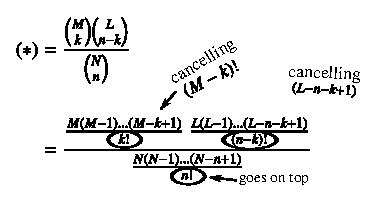
\includegraphics[scale=1.1]{figure/fig3.eps}}

\begin{align*}
(*) &= \dfrac{\binom{M}{k}\binom{L}{n-k}}{\binom{N}{n}}\\
    &= \dfrac{\frac{M(M-1)\ldots (M-k+1)}{k!} \ \frac{L(L-1)\ldots (L-n-k+1)}{(n-k)!}}{\frac{N(N-1)\ldots (N-n+1)}{n!}}
\end{align*}
exercise in fractions
\begin{align*}
& =\dfrac{n!}{k!(n-k)!}\dfrac{M(M-1)\ldots (M-k+1)L(L-1)\ldots (L-n-k+1)}{N(N-1)\ldots (N-n+1)}\\[3pt]
&= \binom{n}{k}\dfrac{M(M-1)\ldots (M-k+1)L(L-1)\ldots (L-n-k+1)}{N(N-1)\ldots (N-n+1)}
\end{align*}
\end{frame}

\begin{frame}
Obviously, the first way (*) is easier so if you are doing a reel-world problem and you start getting things that look like (**) step back and see if you can use the first method instead. You will tend to try the second method first. I will test you on this later.

\smallskip

{\it Prediction} (I was wrong before)

Most of you will use the second (wrong) method.
\end{frame}

\begin{frame}
\myheading{An Important General Problem}

Suppose you draw $n$ chips {\it with replacement} and let $X$ be the number of red chips you get. What distribution does $X$ have?

This explains (a little) the formulas on page 21. Note that if $N$ is far bigger than $n$ then it is almost like drawing with replacement. ``The urn doesn't notice that any chaps have been removed because so few (relatively) have been removed.''
\end{frame}

\begin{frame}
In this case
$$
\dfrac{N-n}{N-1}=\dfrac{N\left(1-\frac{n}{N}\right)}{N\left(1-\frac{1}{N}\right)}\approx \dfrac{N}{N}=1
$$
(because $N$ is huge $\dfrac{1}{N}$ and $\dfrac{n}{N}=0$)

So $V(X)\approx npq$ (see the bottom at pg. 21)

This is what is going on in page 118 of the text.

The number $\dfrac{N-n}{N-1}$ is called the ``finite population correction factor''.
\end{frame}

\end{document}


